% Diese Arbeit beschäftigt sich mit der automatischen Trennung von Schüttgutpartikel.

\section{Einleitung}
Diese Arbeit beschäftigt sich mit der Klassifikation von Schüttgutpartikeln auf Basis von Bewegungsprofilen. Der Begriff Schüttgut bezeichnet hierbei ein körniges oder auch stückiges Gemenge, das in einer schüttfähigen Form vorliegt \cite{SchuettgutDef}. Abbildung \ref{fig:Schuettgut} zeigt Schüttgut in unterschiedlicher Größe. In der Industrie werden Schüttgüter heutzutage maschinell auf Mängel geprüft und automatisch nach Güteklassen getrennt, was die vorherige Klassifikation dieser voraussetzt. Anwendungsgebiete sind vor allem in der Lebensmittelindustrie, beim Recycling oder im Bergbau zu finden. Im Vergleich zur Sortierung per Hand, welche subjektiv und unbeständig ist, hilft die maschinelle Sortierung bei der Erhöhung von Produktqualität und Durchsatz, während Kosten reduziert werden \cite{FoodQuality}.

\begin{figure}[!h]
    \centering
    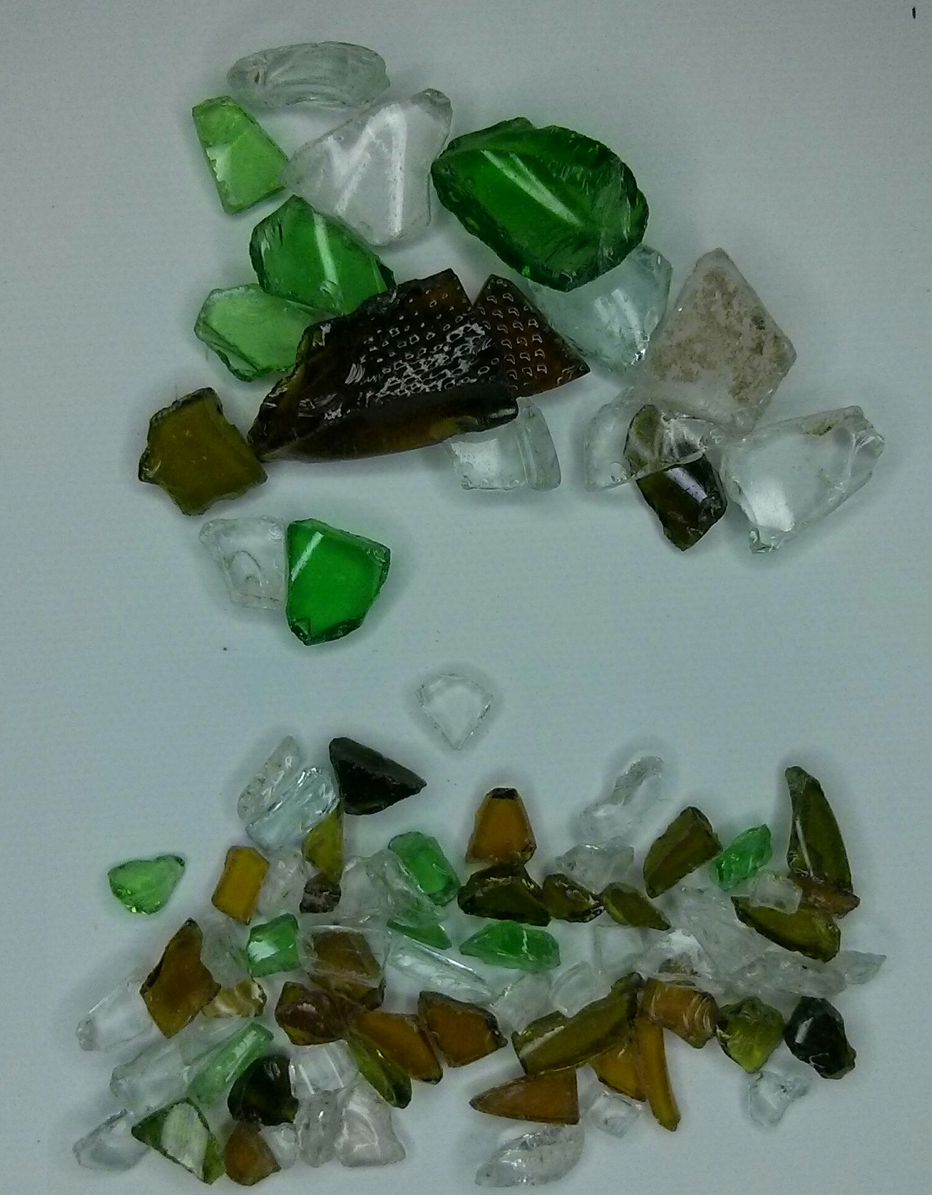
\includegraphics[width=0.3\textwidth]{pics/Schuettgut.png}
    \caption{Schüttgut}
    \label{fig:Schuettgut}
\end{figure}

\subsection{Der sensorbasierte Sortierprozess}
Der sensorbasierte Sortierprozess läuft im Allgemeinen wie in Abbildung \ref{fig:Aufbau} illustriert ab. Schüttgut wird portionsweise an den Anfang eines Fließbandes gestreut und anschließend von diesem beschleunigt. Ein Sensor erfasst relevante Eigenschaften der Schüttgutpartikel auf dem Fließband. Auf Basis dieser Messung werden die Partikel am Ende des Fließbandes in bestimmte Behälter geleitet und so voneinander getrennt.

Bei einem solchen Sensor kann es sich beispielsweise um eine Zeilen- oder Flächenkamera handeln. Die Analyse jedes Partikels durch eine Zeilenkamera beschränkt sich dabei nur auf wenige Bilder. Dadurch ist eine Bewegungsanalyse nicht möglich. Durch geschickte Beleuchtung kann jedoch anhand optischer Merkmale der Partikel eine Klassifikation durchgeführt werden. Mithilfe einer Flächenkamera kann hingegen ein Bewegungsprofil jedes Partikels erfasst und analysiert werden. Partikel unterscheiden sich hierbei nicht nur durch ihren auf dem Band zurückgelegten Pfad, sondern auch hinsichtlich der Geschwindigkeit und Beschleunigungen zu verschiedenen relativen Zeitpunkten.

\begin{figure}[!h]
    \centering
    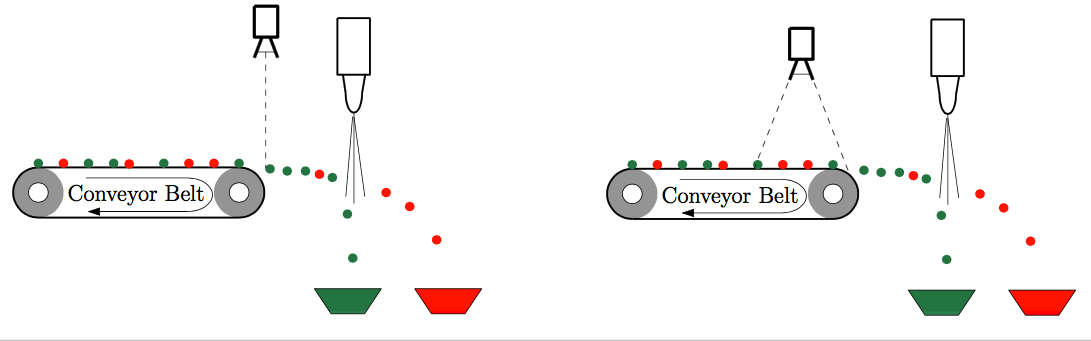
\includegraphics[width=0.7\textwidth]{pics/aufbau.png}
    \caption{Aufbau aus der MA}
    \label{fig:Aufbau}
\end{figure}

\subsection{Motivation}
\label{sec:Motivation}
% Das Ziel dieser Arbeit ist es mithilfe einer Flächenkamera automatisch ein Schüttgut-Partikel abhängig von seinem Bewegungsverlauf zu klassifizieren.
Das Ziel dieser Arbeit ist die Klassifikation von Schüttgutpartikeln auf Basis von Bewegungsprofilen, welche aus den Daten einer Flächenkamera gewonnen werden. Das Erlernen einer akkuraten Klassifikation eines neuen bzw. unbekannten Schüttguts soll dabei schnell und einfach möglich sein.

\subsection{Bisherige Arbeiten}
In der Arbeit \cite{MA} wurde gezeigt, dass auf Basis von Bewegungsprofilen eine Klassifikation von Objekten möglich ist. Als Testdaten wurden dazu mehrere Objektarten verwendet, welche drei Oberklassen zugeordnet werden können. Mithilfe eines naiven Bayes Klassifikators wurden die verschiedenen Objektarten automatisch einer der drei Oberklassen zugeordnet.

Da die Testdaten pro Objektart aus lediglich 52 Objekten bestehen, konnte keine repräsentative Likelihood-Funktion umgesetzt werden \cite[S. 24]{MA}. Außerdem wurde festgestellt, dass manche Objektarten ein sehr ähnliches Bewegungsverhalten aufweisen. Unter der Berücksichtigung der genannten Einschränkungen konnte in durchschnittlich 90\% der Fällen eine korrekte Zuordnung der Objekte zur Oberklasse erreicht werden \cite[S. 24]{MA}. Die Arbeit kommt zum Schluss, dass durch die Verwendung größerer Testdatenmengen und Features ein besseres Klassifikationsergebnis erreicht werden kann.

\subsection{Zielsetzungen}
\label{sec:Goal}
Es soll ein Klassifikator entwickelt werden, welcher Schüttgutpartikel verschiedener Schüttgutarten mit einer Genauigkeit von mehr als 90\% trennt. Dabei soll der Klassifikator nicht nur (wie in \cite{MA} umgesetzt) zwischen Oberklassen, sondern auch zwischen Basisklassen unterscheiden können. Der Klassifikator soll dazu möglichst wenige Realdaten benötigen und keine optischen Merkmalen, sondern ausschließlich Daten aus dem Bewegungsprofil für seine Entscheidung nutzen. Die spätere Umsetzung des Klassifikators soll durch die Optimierung der Anlagenparameter außerdem eine Klassifikation in Echtzeit ermöglichen.




